% File tacl2018v2.tex
% Sep 20, 2018

% The English content of this file was modified from various *ACL instructions
% by Lillian Lee and Kristina Toutanova
%
% LaTeXery is mostly all adapted from acl2018.sty.

\documentclass[11pt,a4paper]{article}
\usepackage{times,latexsym}
\usepackage{url}
\usepackage[T1]{fontenc}
\usepackage{graphicx}
%% Package options:
%% Short version: "hyperref" and "submission" are the defaults.
%% More verbose version:
%% Most compact command to produce a submission version with hyperref enabled
%%    \usepackage[]{tacl2018v2}
%% Most compact command to produce a "camera-ready" version
%%    \usepackage[acceptedWithA]{tacl2018v2}
%% Most compact command to produce a double-spaced copy-editor's version
%%    \usepackage[acceptedWithA,copyedit]{tacl2018v2}
%
%% If you need to disable hyperref in any of the above settings (see Section
%% "LaTeX files") in the TACL instructions), add ",nohyperref" in the square
%% brackets. (The comma is a delimiter in case there are multiple options specified.)

\usepackage[acceptedWithA]{tacl2018v2}




%%%% Material in this block is specific to generating TACL instructions
\usepackage{xspace,mfirstuc,tabulary}
\newcommand{\dateOfLastUpdate}{Sept. 20, 2018}
\newcommand{\styleFileVersion}{tacl2018v2}

\newcommand{\ex}[1]{{\sf #1}}

\newif\iftaclinstructions
\taclinstructionsfalse % AUTHORS: do NOT set this to true
\iftaclinstructions
\renewcommand{\confidential}{}
\renewcommand{\anonsubtext}{(No author info supplied here, for consistency with
TACL-submission anonymization requirements)}
\newcommand{\instr}
\fi

%
\iftaclpubformat % this "if" is set by the choice of options
\newcommand{\taclpaper}{final version\xspace}
\newcommand{\taclpapers}{final versions\xspace}
\newcommand{\Taclpaper}{Final version\xspace}
\newcommand{\Taclpapers}{Final versions\xspace}
\newcommand{\TaclPapers}{Final Versions\xspace}
\else
\newcommand{\taclpaper}{submission\xspace}
\newcommand{\taclpapers}{{\taclpaper}s\xspace}
\newcommand{\Taclpaper}{Submission\xspace}
\newcommand{\Taclpapers}{{\Taclpaper}s\xspace}
\newcommand{\TaclPapers}{Submissions\xspace}
\fi
\setcounter{secnumdepth}{4}
%%%% End TACL-instructions-specific macro block
%%%%

\title{IMapbook: Automating Analysis of Group Discussions}


% Author information does not appear in the pdf unless the "acceptedWithA" option is given
% See tacl2018v2.sty for other ways to format author information
\author{Patrik Kojanec \and Marko Rus}
% todo: naslovi

\date{}

\begin{document}
\maketitle

% \begin{abstract} 
% \end{abstract}

\section{Introduction}
Nature Language Processing has seen a huge rise in popularity in recent years. It is now broadly studied topic with many successful applications. In this project we touch subfield Text Classification and apply its methods to the data from IMapbook \cite{imapbook}, a web-based technology that allows reading material to be intermingled with interactive games and discussions. Some portion of discussions from this platform were manually annotated, each reply was given more categories based on the information in the reply. Our goal is to  take this data and try to build a classifier which would predict these categories. Such classifier could then be used to automate analysis of discussions at this platform, recommend the time for the teacher’s intervention and more.

\subsection{Related work}
The domain of our problem is short-text classification, which is closely related to social media. Unlike the common text classification problems, where the documents are usually long and written in formal language, it deals with texts of few sentences, written in informal language. The amount of context information carried in the texts is usually very low, thus classification and information retrieval become challenging tasks to perform efficiently \cite{Song2014}. Furthermore, the low co-occurrence of words induced by the shortness of the texts often results problematic for machine learning algorithms, which rely on word frequency.\\
With the arise of social media this branch of text classification became a well researched problem, and people tried different approaches to overcome its constraints. In a survey in 2014, \cite{Song2014} pointed out the main methods of short text classification, which mostly relate on semantic analysis, since it pays more attention to the concept, inner structure semantic level, and the correlation of texts to obtain the logic structure, which is more expressive and objective. Currently, the most widely used vector representations of words (or embeddings), that proved to capture well the semantic information are GloVE \cite{glove2014} and Word2Vec \cite{word2vec}.\\
Although standard machine learning approaches often resulted problematic with short text, Sriram et al. \cite{Sriram2010} showed that their model with hand-crafted features, related to user's tweets\footnote{Short text message on the Twitter platform (www.twitter.com).}, efficiently filtered irrelevant tweets from the users, thus suggesting that by adding extra sources of context information increases the performance. Similarly, this concept was also recently shown by Yang et al. \cite{Yang2018}. Furthermore, they have also shown that Support Vector Machines performed almost equally well in classification when using word embeddings or TF-IDF, but they were outperformed by deep neural networks.\\
%Furthermore, they have also presented some examples of short text classification using ensemble classifiers, which outperformed traditional machine learning methods.\\
%\cite{Yang2018} \cite{Choudhury2015}.

\section{Dataset}
\label{dataset}
The dataset is provided by IMapBook and includes the discussions between students and teachers on the topics of the book they are reading. The dataset includes approximately 3500 Slovene messages, from 9 different schools and on 7 different books, which were also translated to English. Students in each school were divided in "book clubs", where the conversations occurred.\\
The data was manually annotated, with three main tags:
\begin{itemize}
    \item \textit{Book Relevance}: Whether the content of the message is relevant to the topic of the book discussion.
    \item \textit{Type}: Whether the message is a question (Q), answer (A) or a statement (S). In original data mixture of these classes also appear (QA and AQ), but because of their low frequency (together they appear only three times in entire dataset), we changed QA occurrences to Q and AQ to A.
    \item \textit{Category}: Whether the message is a simple chat message (C), related to the book discussion (D), moderating the discussion (M), wondering about users' identities (I), referring to a task, switching it or referring to a particular position in the application (S), or other cases (O).
\end{itemize}
The \textit{Category} category can be further on split in sub-categories; \textit{chats} may be in the form of greetings (G), related to the book (B), they could be encouraging (E), talk about feelings (F), contain cursing (C) or others (O), \textit{Discussion} messages could be questions (Q), answers (A), answers to users, still related to the discussion topic (AA) or encouraging the discussion (E); \textit{identity} messages can be answers(A), questions (Q) or their combination (QA).\\
The dataset is suitable for both binary and multi-class classification, whether the target variable is the relevance or the category of the message respectively.\\

\section{Methods}
In this section we present the methods that will be used to perform three different message classification tasks:
\begin{enumerate}
    \item Book relevance classification (binary)
    \item Type of message classification (3-class)
    \item Broad category classification (6-class)
\end{enumerate}

Input data to all classifiers (except for Majority Classifier) are questions and answers in Slovenian.

\subsection{Baseline}
As a baseline model we decided to use Majority Classifier. In each task it classifies every instance as the most representative class in training set.

\subsection{Hand-Crafted Feature Models}
The first group of models that we present is based on a hand-crafted feature set. These features were then used as an input to different classification algorithms, that we list in Section~\ref{sssc:class-alg}. We describe features extraction in the next section.

\subsubsection{Features Extraction}
The aim of the features was to simply and intuitively capture the relevance to the question, while filtering gibberish and inappropriate messages. Thus, the following set of features was designed:

\begin{itemize}
     \item Number of tokens in a message.
     \item Number of mistakes in a message; this was computed by matching words with the words in a lexicon \cite{11356/1230}.
     \item Maximal length of the token in the message.
     \item Number of characters in a message.
     \item Number of question marks in a message.
     \item Number of exclamation points in a message.
     \item Number of commas in a message.
     \item Number of periods in a message.
     \item Number of capital letters in a message.
     \item Number of capital letters within the interior of the words  in a message.
     \item Number of peculiar characters in a message.
     \item Number of numbers within the interior of the words in a message.
     \item \textit{Levenshtein distance:} Number of all pairs of words from the question and the message, whose Levenshtein distance is less than half the length of the longest of the two words.
     \item Number of interrogative words in a message.
     \item Number of 'kdo' in a message.
\end{itemize}

In the case of \textit{Levenshtein distance} feature,  the messages were initially tokenized and stop-words \cite{sloStopWords} were removed, while for other cases regular expressions were used to extract the features.

All features designed while looking at the data, having some sense in how the feature could increase the classification success. For instance, many messages  had 'kdo' word in it, asking for identity of somebody. Those messages have the same class. But nevertheless we observed only small portion of the data, so that chosen features would not be overfitted.

\subsubsection{Classification Algorithms}
\label{sssc:class-alg}
We decided to feed the features to four different classification algorithms to see how they perform. We chose a na\^ive bayesian (NB), random forest (RF), support vector machine (SVM) and a logistic regression (LR) classifiers. We used the implementations from scikit-learn library \cite{scikit-learn}.

When selecting the parameters we observed train and test error and paid closed attention to detecting overfitting. For NB we left the default parameters. For the SVM we used the RBF kernel and set the parameter \textit{gamma} to 'auto' and \textit{C} to 5, while for the LR we decided to use 'lbfgs' optimizer with maximum 1000 iterations. In the case of LR the input data was standardized to prevent numerical instabilities. For the RF we set the number of estimators to 150, while \textit{min\_samples\_leaf} to 3 and \textit{min\_samples\_split} to 10. This way we managed to reduce the overfitting to the training data. We kept the same parameters for all the tasks.

\section{Evaluation}
To evaluate the performance we decided to use the classification accuracy as evaluation metrics.\textbf{TODO: why accuracy?} We used 5-fold cross validation on the whole dataset, where our performance estimator was the average result of the five test sets. The results are presented in the next section.

\section{Results}
In Figure \ref{fig:acc_res}, we notice that all feature-based classifiers outperform the majority classifier. Furthermore, as expecting, the classification accuracy drops with increasing number of target classes. The best performing classification algorithm on this dataset seems to be the random forest, which outperformed the others in both 'CategoryBroad' and 'Type' classification tasks. Its performance on the 'Book Relevance' task was also on average higher than the rest, however SVM and LR obtained comparable results. Surprisingly, LR with multi-class extension, performed quite well also on multi-class classification tasks.\\
Initially, RF yielded very high performance on the training set, reaching a 95\% accuracy. However, the performance on the test set was lower, showing signs of overfitting. Thus, with a more careful selection of the parameters, we dropped the training accuracy for about 10\% and reached the current test performance.\\
\begin{figure}[h]
    \centering
    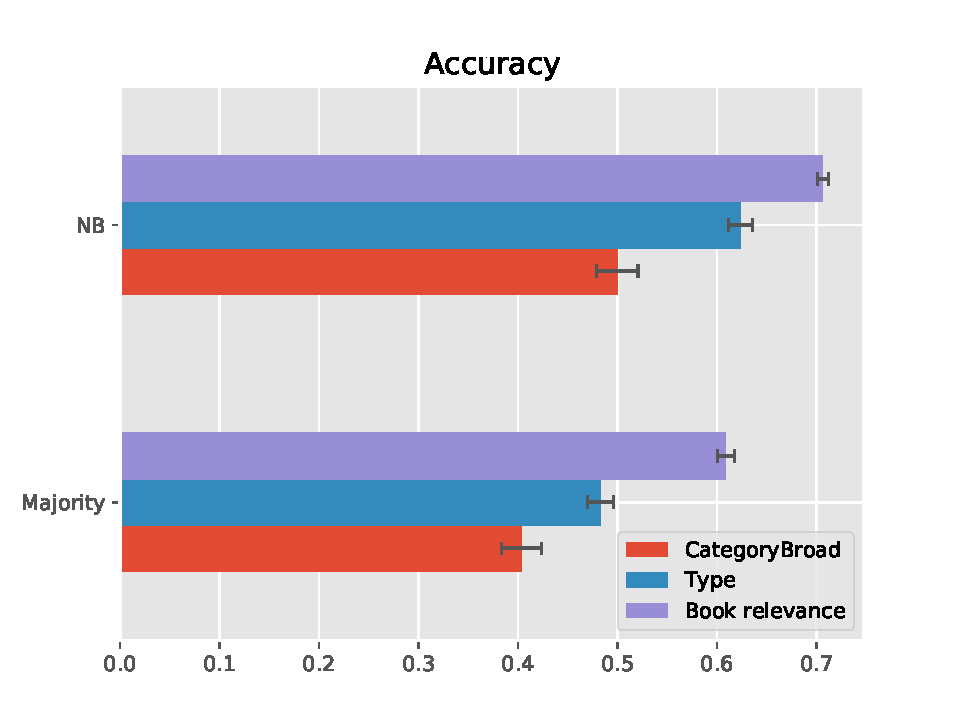
\includegraphics[width = \linewidth]{../results/Accuracy_plot.pdf}
    \caption{\textbf{Accuracy evaluation.} Classification accuracy of the models on three different classification tasks described in Section \ref{dataset}.}
    \label{fig:acc_res}
\end{figure}

\section{Discussion and Future Perspective}
Random forest seems to be a very powerful classification algorithm that really well fits the given data. However, a careful tuning is needed to prevent overfitting. Furthermore, RF is often used as a feature selection tool, as it ranks the importance of the features. In Figure \ref{fig:ft_imp_RF} we show the importance of each feature in the decision process of the RF model.
\begin{figure}[h]
    \centering
    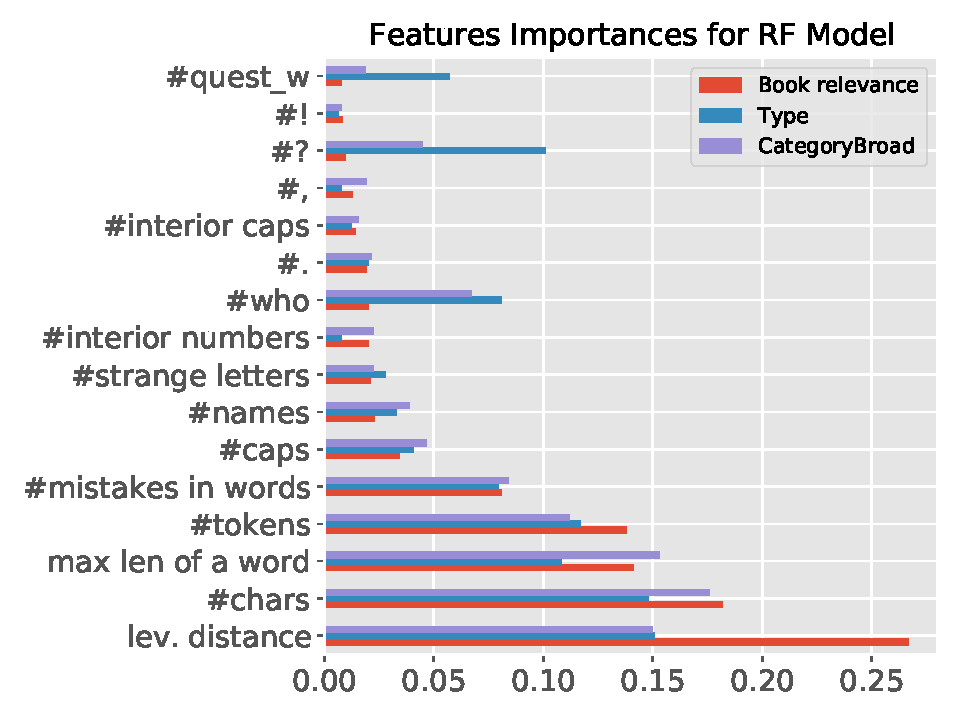
\includegraphics[width = \linewidth]{../results/feature_imp_RF_plot.pdf}
    \caption{\textbf{Feature Importance for RF.} This plot sh.}
    \label{fig:ft_imp_RF}
\end{figure}
As we notice, each classification tasks focuses on different features, however there are some common one that are discriminatory for all three tasks, i.e. last five in the plot. As expected, \textit{Lev. distance} works particularly well on the 'Book relevance' problem, since it performs a naive kind of matching of the text messages with the questions. However, it results also as the most discriminatory feature for 'Type' classification and third for 'CategoryBroad' classification.\\
It is not surprising that some features are particularly relevant to some classification task, since they were designed for that purpose. It is also known that good features increase performance. Here we showed that some features are particularly suitable for some specific tasks, while others behave well over different classification problems. One future improvement that could be done is trying to define some other features that would boost the performance, removing the irrelevant ones. \\

%\subsection{Further Work}
% Our goal is to construct and implement a model for predicting relevancy of replies and their category, based on the dataset from IMapbook (see Section~\ref{dataset}). Due to relatively small size of the dataset, models based on neural networks can not be trained, and pre-trained models are not an option because of the vivid language used in conversations. Throughout the work we will only use original (Slovene) replies and ignore English translations, because they were not automatically generated. 

% Keeping above in mind our work can be divided into three main categories:

% \begin{enumerate}
%   \item \textit{Data Preprocessing}:  Due to many errors in the language, intensive preprocessing is required. Many words are from the Slovene dictionary, and first thing to do would be to classify these words, for instance into mistakes, slang and gibberish. For other words regular text normalization will be applied.
%   \item \textit{Feature Extraction}: Many features will be hand-crafted, based on the presence of the certain symbols, lengths of words, number of correctly spelled words, number of messages by that person up to observed reply, and so on.
%   \item \textit{Model Fitting \& Evaluation}: We will try more models, such as Naive Bayes \cite{bayes}, Logistic Regression \cite{kleinbaum2002logistic}, Support-Vector Machines \cite{joachims2002learning}, Random Forest \cite{liaw2002classification}, and evaluate them by accuracy and F measure.
% \end{enumerate}




% \begin{table}[t]
% \begin{center}
% \begin{tabular}{|l|rl|}
% \hline \bf Type of Text & \bf Size & \bf Style \\ \hline
% paper title & 15 pt & bold \\
% \iftaclpubformat
% author names & 12 pt & bold \\
% author affiliation & 12 pt & \\
% \else
% \fi
% the word ``Abstract'' as header & 12 pt & bold \\
% abstract text & 10 pt & \\
% section titles & 12 pt & bold \\
% document text & 11 pt  &\\
% captions & 10 pt & \\
% %bibliography & 10 pt & \\
% footnotes & 9 pt & \\
% \hline
% \end{tabular}
% \end{center}
% \caption{\label{tab:font-table} Font requirements}
% \end{table}


\bibliography{tacl2018}
\bibliographystyle{acl_natbib}

\end{document}


